\chapter{Datenbank}
\newcounter{ids}

   In diesem Abschnitt wird beschrieben, wie die Daten in einer relationaler Datenbank aussehen werden. Die Umwandlung aus den Django Modellen in die relationalen Tabellen wird von dem ORM (Object Relational Mapping) Modul realisiert, das von Django bereitgestellt wird. Django unterstützt mehrere moderne Datenbanksysteme, was bedeutet, dass die Datenbank austauschbar ist. Im folgenden (Abbildung \ref{fig:er_diagramm}) sind die Entitäten und deren Beziehungen dargestellt. 

    \begin{figure}[h]
        \centering
        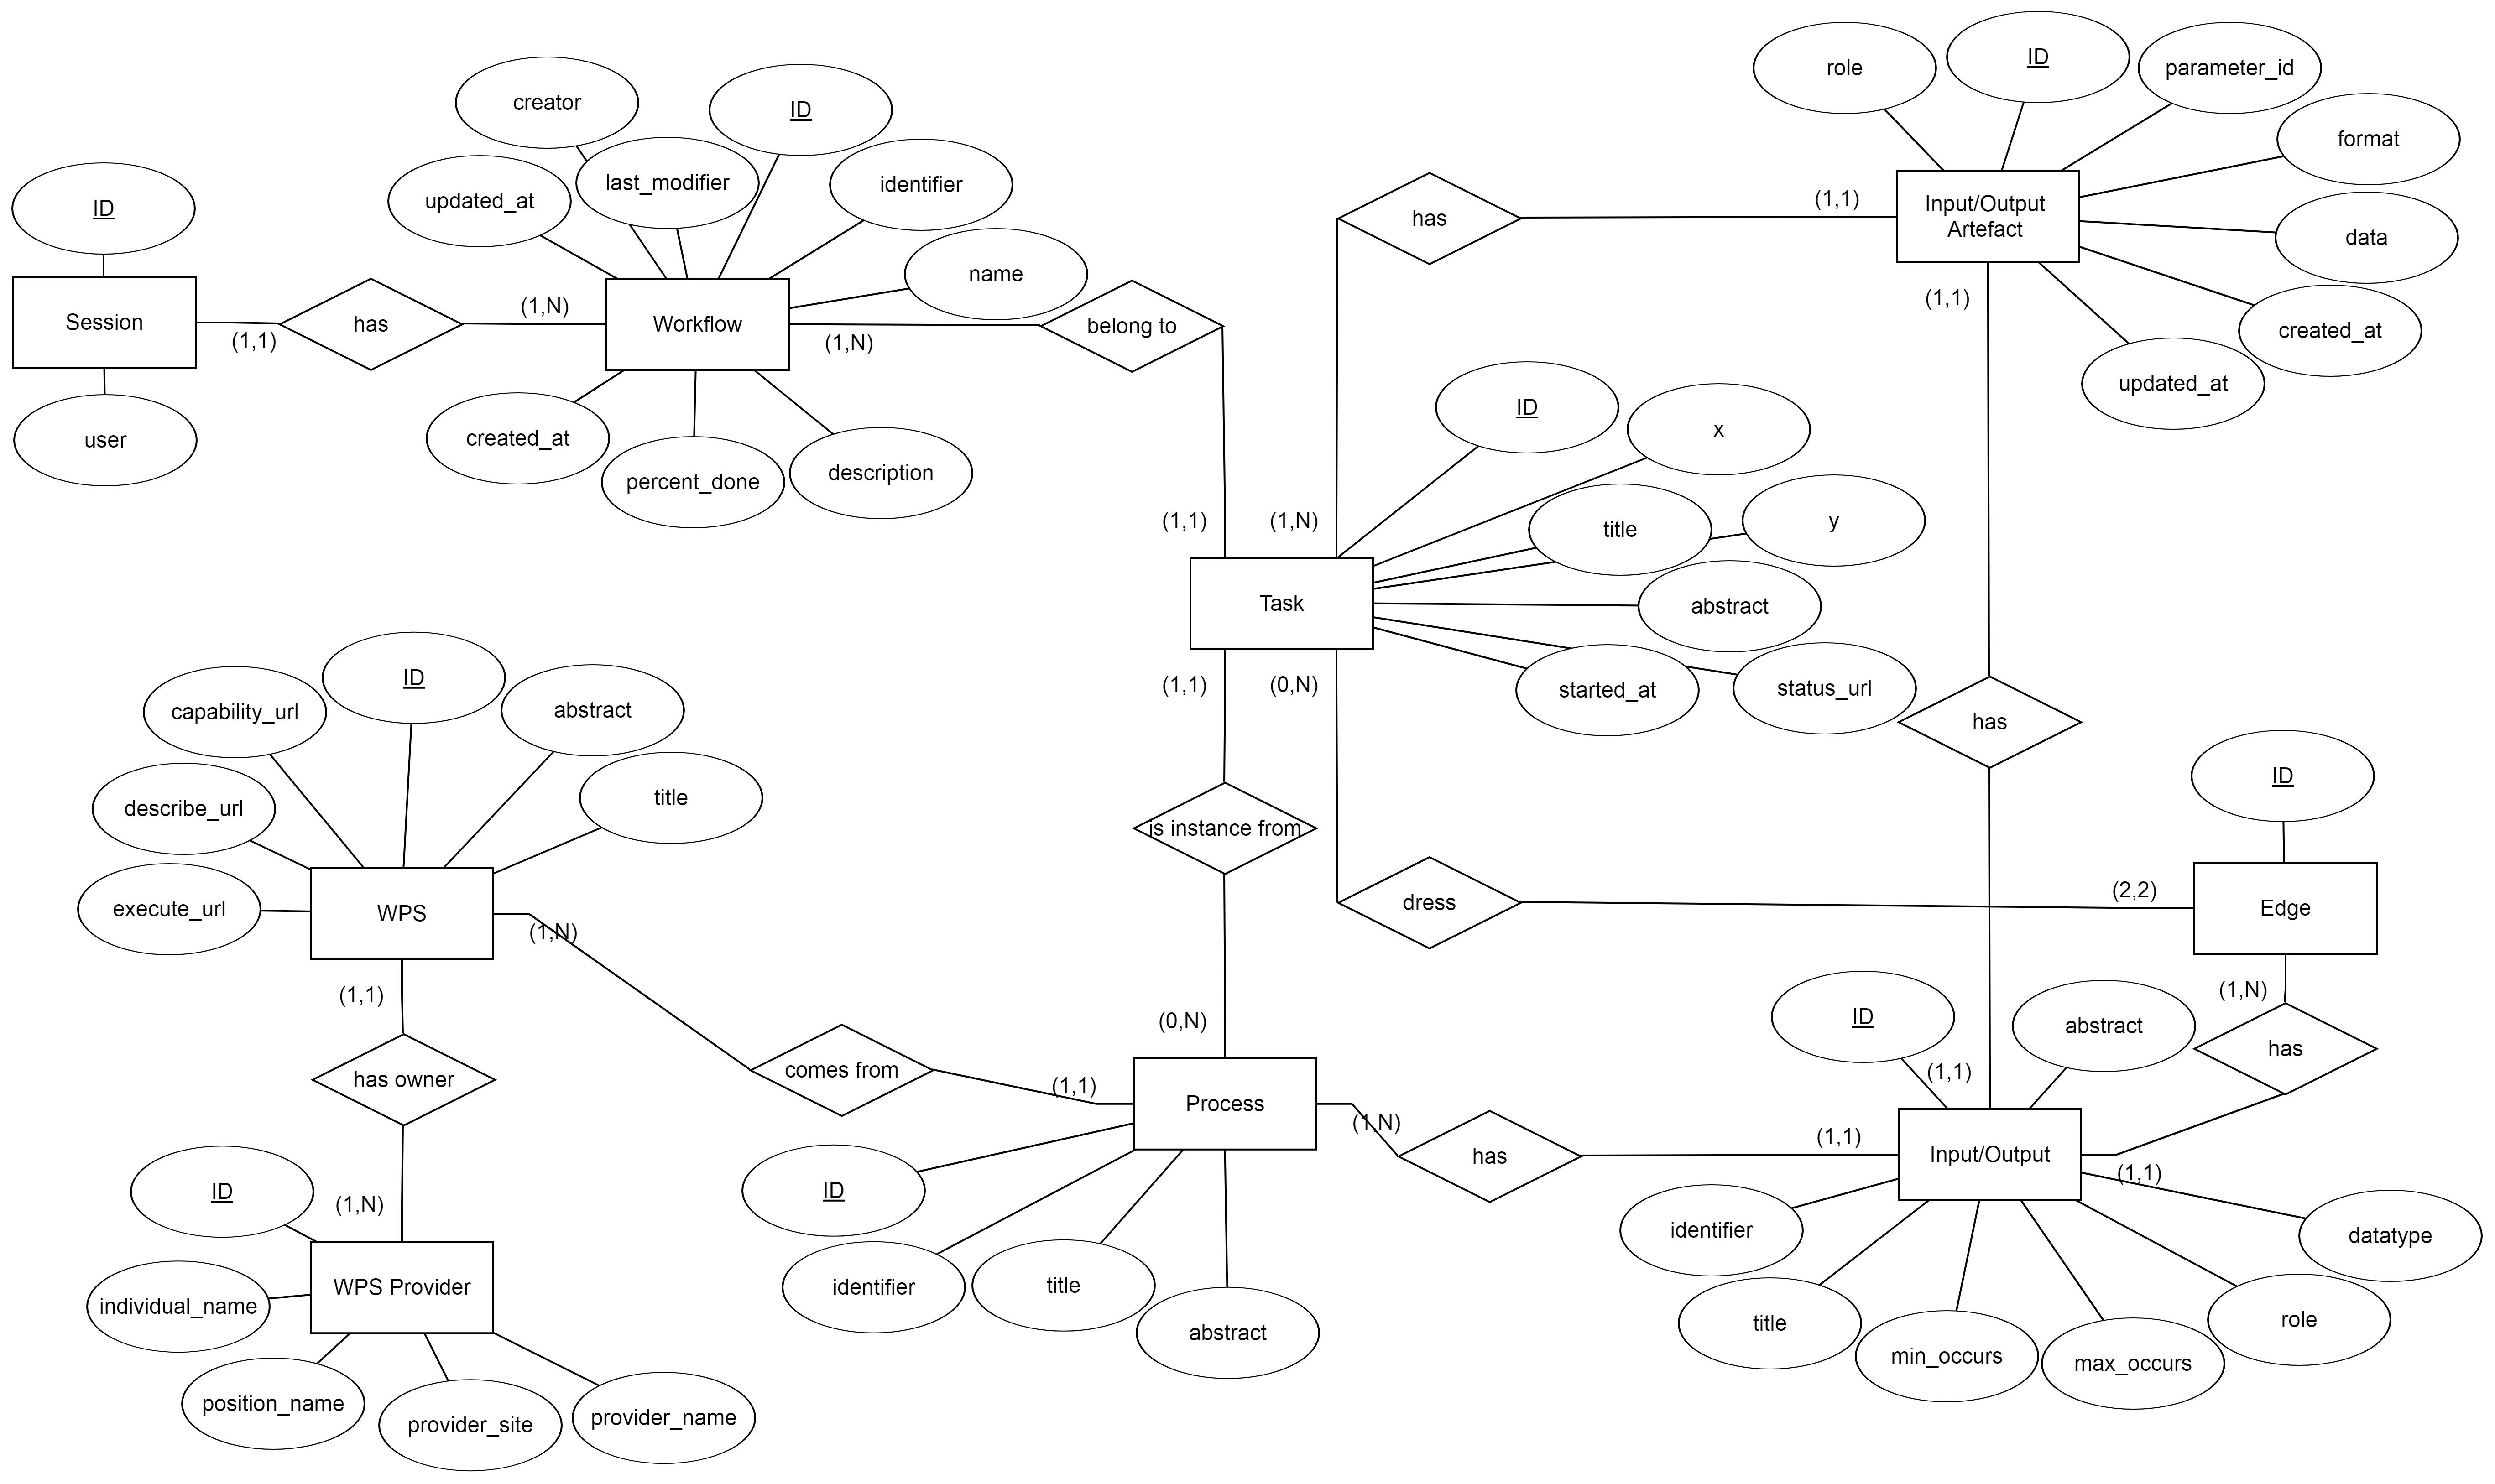
\includegraphics[width=15cm]{diagrams/ERDiagramm.png}
        \caption{Entity Relationship Diagram}
        \label{fig:er_diagramm}
    \end{figure}
	
	
	\section{Tabellen}
	
	    Im folgenden finden Sie den Aufbau der Tabellen wie sie in der Datenbank zu finden sein werden.\newline
	
 		\subsection{Session}
 		\begin{center}
 			\setlength\tabcolsep{5pt}
 			\renewcommand{\arraystretch}{1.5}
 			\setcounter{ids}{0}			
 			\begin{tabular}{|c|c|c|}
 				\hline
 				\rowcolor[gray]{0.75}[4.85pt]
 				id & user\_id & last\_workflow\_id \\ \hline  
 				&& \\	
 				\hline
 			\end{tabular}
 		\end{center}		


 		\subsection{WPSProvider}
 		\begin{center}
 			\setlength\tabcolsep{5pt}
 			\renewcommand{\arraystretch}{1.5}
 			\setcounter{ids}{0}			
 			\begin{tabular}{|c|c|c|c|c|}
 				\hline
 				\rowcolor[gray]{0.75}[4.85pt]
 				id & provider\_name & provider\_site & individual\_name & position\_name \\ \hline  
 				&&&& \\	
 				\hline
 			\end{tabular}
 		\end{center}		


		\subsection{Edge}
		\begin{center}
			\setlength\tabcolsep{5pt}
			\renewcommand{\arraystretch}{1.5}
			\setcounter{ids}{0}			
			\begin{tabular}{|c|c|c|c|c|c|}
				\hline
				\rowcolor[gray]{0.75}[4.85pt]
				id & workflow & from\_task\_id & to\_task\_id & input\_id & output\_id \\ \hline
				&&&&& \\	
				\hline
			\end{tabular}
		\end{center}		
		
		\subsection{Process}
		\begin{center}
			\setlength\tabcolsep{5pt}
			\renewcommand{\arraystretch}{1.5}
			\setcounter{ids}{0}			
			\begin{tabular}{|c|c|c|c|c|}
				\hline
				\rowcolor[gray]{0.75}[4.85pt]
				id & wps\_id & identifier & title & abstract \\ \hline  
				&&&& \\	
				\hline
			\end{tabular}
		\end{center}		
		

		\subsection{WPS}   
		\begin{center}
			\setlength\tabcolsep{5pt}
			\renewcommand{\arraystretch}{1.5}
			\setcounter{ids}{0}			
			\begin{tabular}{|c|c|c|c|c|c|c|}
				\hline
				\rowcolor[gray]{0.75}[4.85pt]
				id & service\_provider\_id & title & capabilities\_url & describe\_url & execute\_url & abstract \\ \hline
				&&&&&& \\
				\hline
			\end{tabular}
		\end{center}

		\subsection{Task}
		\begin{center}
			\setlength\tabcolsep{5pt}
			\renewcommand{\arraystretch}{1.5}
			\setcounter{ids}{0}			
			\begin{tabular}{|c|c|c|c|c|c|c|c|c|c|}
				\hline
				\rowcolor[gray]{0.75}[4.85pt]
				id & workflow\_id & process\_id & x & y & status & title & status\_url & started\_at & abstract \\ \hline
				&&&&&&&&& \\
				\hline
			\end{tabular}
		\end{center} 
		
		
		\subsection{Workflow}
		\begin{center}
			\setlength\tabcolsep{5pt}
			\renewcommand{\arraystretch}{1.5}
			\setcounter{ids}{0}			
			\begin{tabular}{|c|c|c|c|c|c|c|c|}
				\hline
				\rowcolor[gray]{0.75}[4.85pt]
				id & name & percent\_done & created\_at & updated\_at & creator\_id & last\_modifier_id & description \\ \hline 
				&&&&&&& \\
				\hline
			\end{tabular}
		\end{center}
		
		
		
		\subsection{InputOutput}
		\begin{center}
			\setlength\tabcolsep{5pt}
			\renewcommand{\arraystretch}{1.5}
			\setcounter{ids}{0}			
			\begin{tabular}{|c|c|c|c|c|c|c|c|c|}
				\hline
				\rowcolor[gray]{0.75}[4.85pt]
				id & process\_id & role & identifier & title & datatype & min\_occurs & max\_occurs & abstract \\ \hline 
				&&&&&&&& \\
				\hline
			\end{tabular}
		\end{center}
		
		
		\subsection{Artefact}
		\begin{center}
			\setlength\tabcolsep{5pt}
			\renewcommand{\arraystretch}{1.5}
			\setcounter{ids}{0}			
			\begin{tabular}{|c|c|c|c|c|c|c|c|}
				\hline
				\rowcolor[gray]{0.75}[4.85pt]
				id & task\_id & parameter\_id & role & format & data & created\_at & updated\_at \\ \hline 
				&&&&&&& \\
				\hline
			\end{tabular}
		\end{center}